% Graphic for TeX using PGF
% Title: /home/lsmael/Ajedrez.dia
% Creator: Dia v0.97.1
% CreationDate: Tue Dec  6 12:45:41 2011
% For: lsmael
% \usepackage{tikz}
% The following commands are not supported in PSTricks at present
% We define them conditionally, so when they are implemented,
% this pgf file will use them.
\ifx\du\undefined
  \newlength{\du}
\fi
\setlength{\du}{15\unitlength}
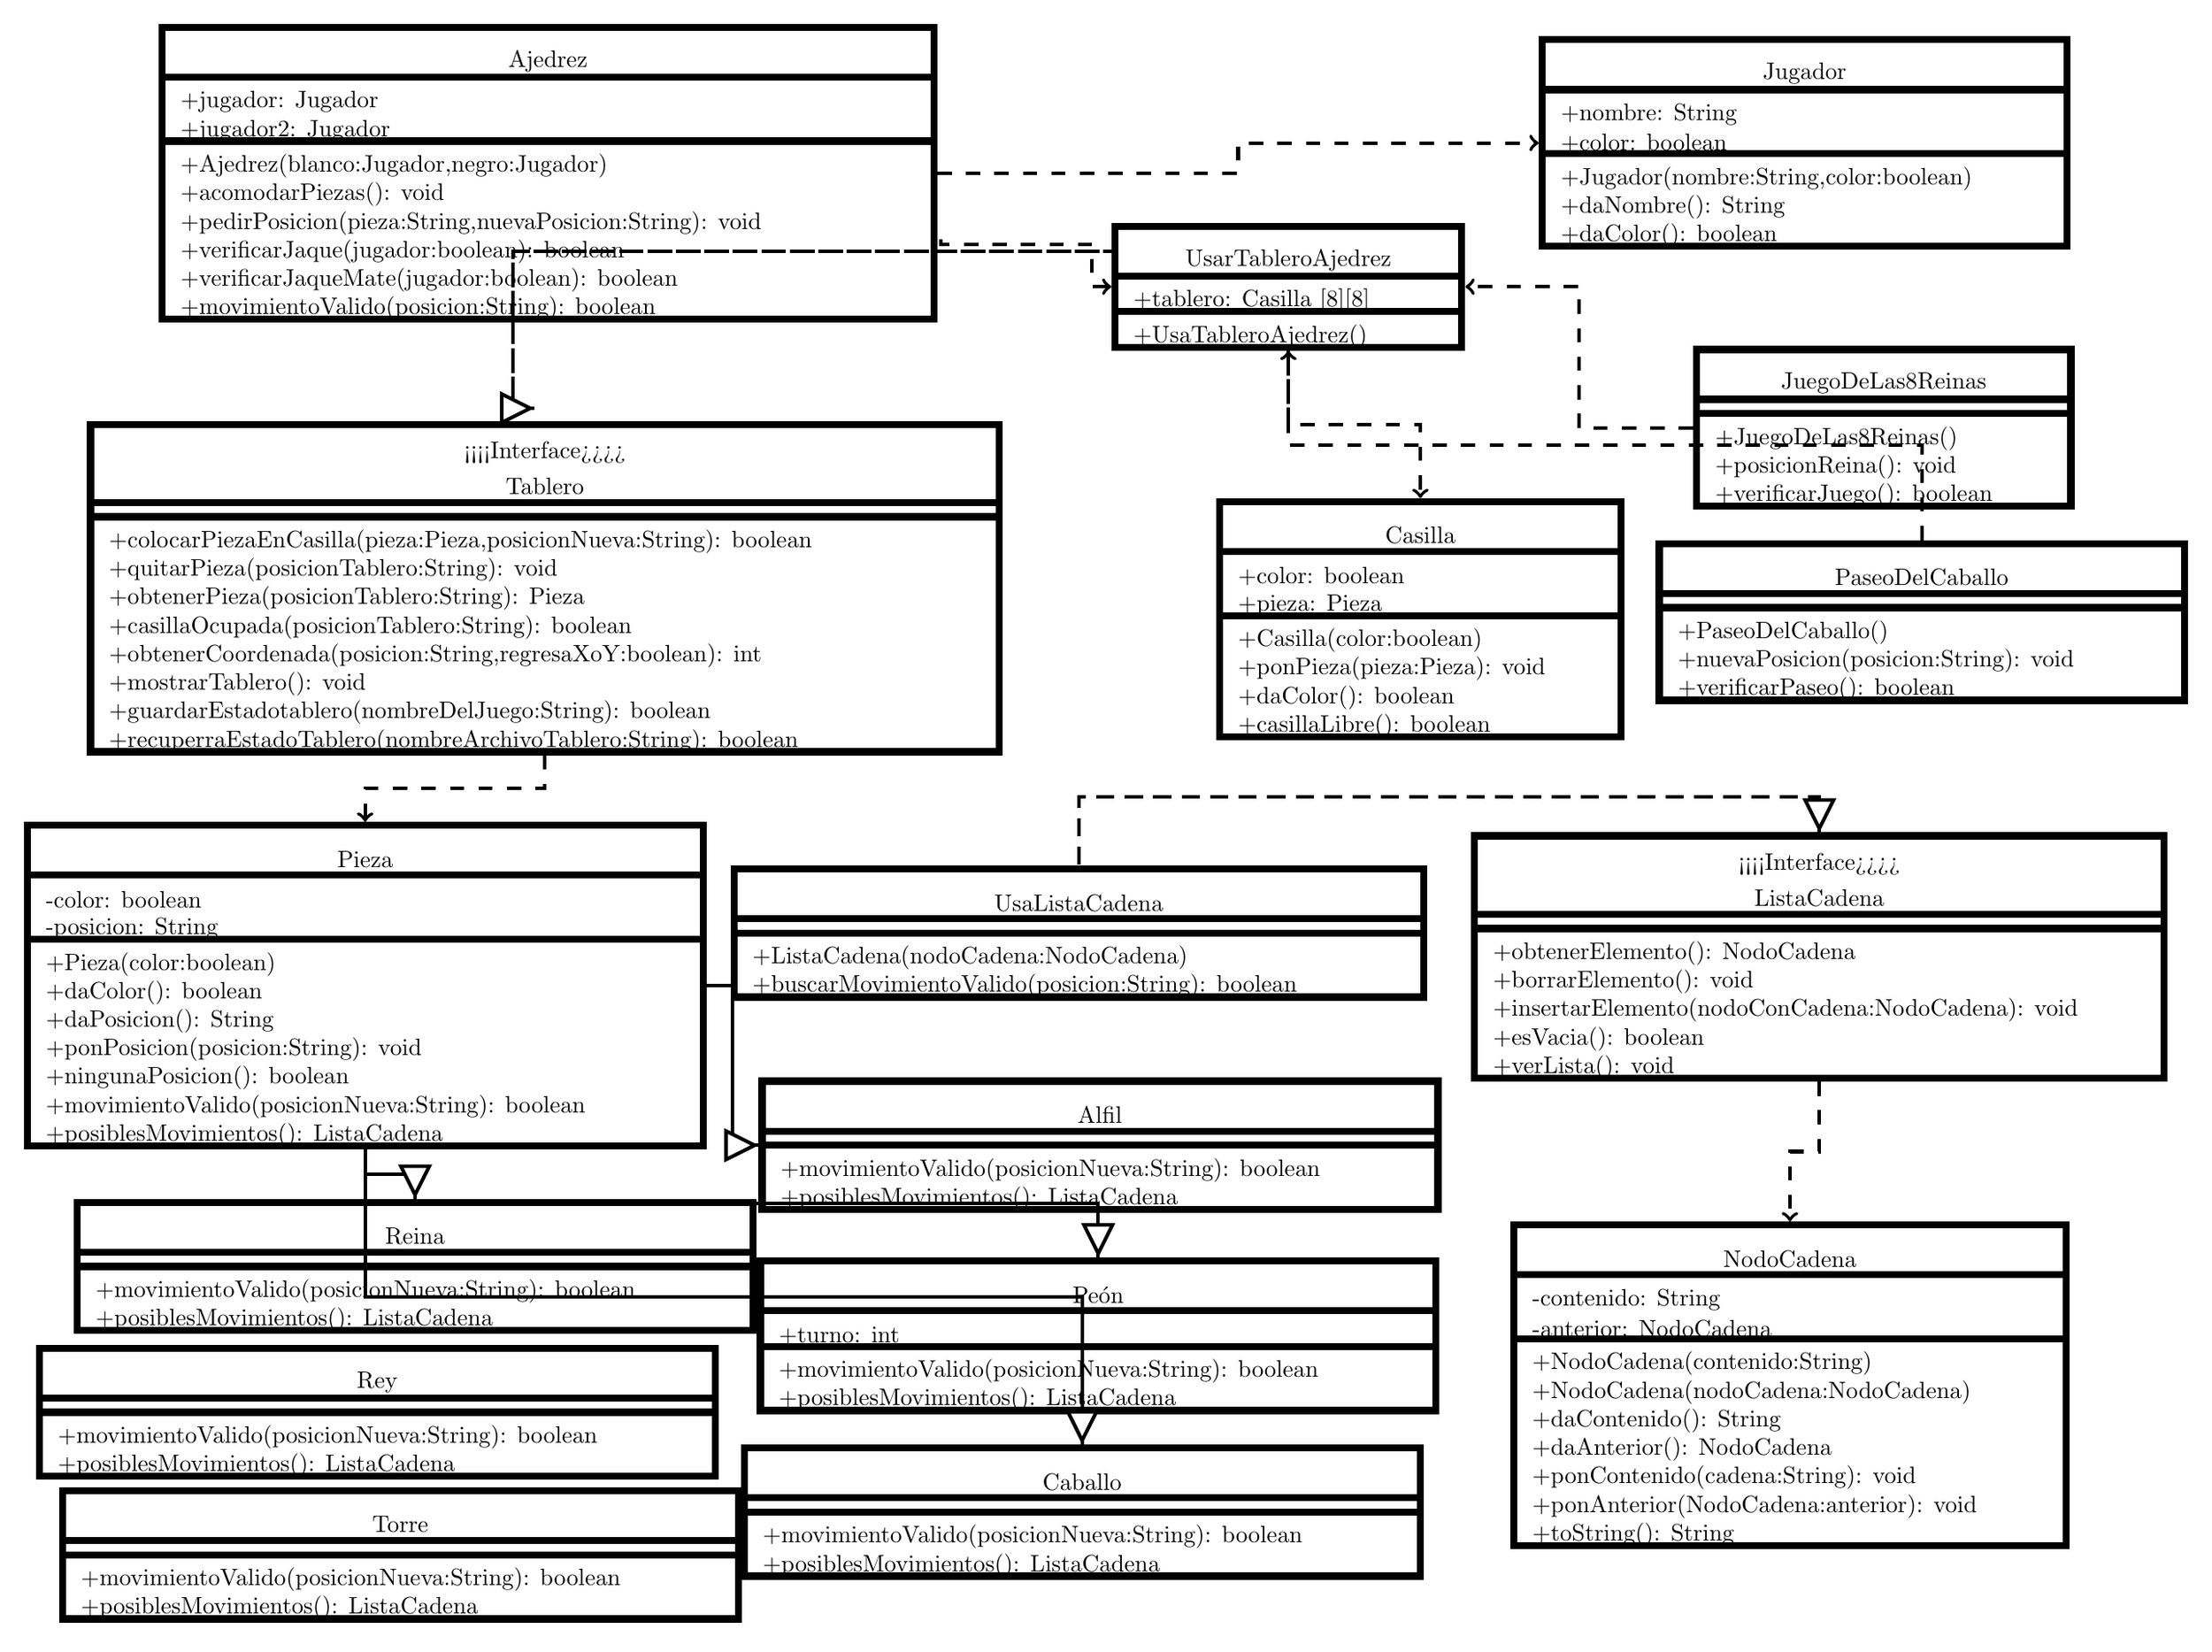
\begin{tikzpicture}
\pgftransformxscale{1.000000}
\pgftransformyscale{-1.000000}
\definecolor{dialinecolor}{rgb}{0.000000, 0.000000, 0.000000}
\pgfsetstrokecolor{dialinecolor}
\definecolor{dialinecolor}{rgb}{1.000000, 1.000000, 1.000000}
\pgfsetfillcolor{dialinecolor}
\pgfsetlinewidth{0.200000\du}
\pgfsetdash{}{0pt}
\definecolor{dialinecolor}{rgb}{1.000000, 1.000000, 1.000000}
\pgfsetfillcolor{dialinecolor}
\fill (17.300000\du,-20.400000\du)--(17.300000\du,-18.200000\du)--(42.825000\du,-18.200000\du)--(42.825000\du,-20.400000\du)--cycle;
\definecolor{dialinecolor}{rgb}{0.000000, 0.000000, 0.000000}
\pgfsetstrokecolor{dialinecolor}
\draw (17.300000\du,-20.400000\du)--(17.300000\du,-18.200000\du)--(42.825000\du,-18.200000\du)--(42.825000\du,-20.400000\du)--cycle;
% setfont left to latex
\definecolor{dialinecolor}{rgb}{0.000000, 0.000000, 0.000000}
\pgfsetstrokecolor{dialinecolor}
\node at (30.062500\du,-19.600000\du){<<<<Interface>>>>};
% setfont left to latex
\definecolor{dialinecolor}{rgb}{0.000000, 0.000000, 0.000000}
\pgfsetstrokecolor{dialinecolor}
\node at (30.062500\du,-18.650000\du){Tablero};
\definecolor{dialinecolor}{rgb}{1.000000, 1.000000, 1.000000}
\pgfsetfillcolor{dialinecolor}
\fill (17.300000\du,-18.200000\du)--(17.300000\du,-17.800000\du)--(42.825000\du,-17.800000\du)--(42.825000\du,-18.200000\du)--cycle;
\definecolor{dialinecolor}{rgb}{0.000000, 0.000000, 0.000000}
\pgfsetstrokecolor{dialinecolor}
\draw (17.300000\du,-18.200000\du)--(17.300000\du,-17.800000\du)--(42.825000\du,-17.800000\du)--(42.825000\du,-18.200000\du)--cycle;
\definecolor{dialinecolor}{rgb}{1.000000, 1.000000, 1.000000}
\pgfsetfillcolor{dialinecolor}
\fill (17.300000\du,-17.800000\du)--(17.300000\du,-11.200000\du)--(42.825000\du,-11.200000\du)--(42.825000\du,-17.800000\du)--cycle;
\definecolor{dialinecolor}{rgb}{0.000000, 0.000000, 0.000000}
\pgfsetstrokecolor{dialinecolor}
\draw (17.300000\du,-17.800000\du)--(17.300000\du,-11.200000\du)--(42.825000\du,-11.200000\du)--(42.825000\du,-17.800000\du)--cycle;
% setfont left to latex
\definecolor{dialinecolor}{rgb}{0.000000, 0.000000, 0.000000}
\pgfsetstrokecolor{dialinecolor}
\node[anchor=west] at (17.500000\du,-17.100000\du){+colocarPiezaEnCasilla(pieza:Pieza,posicionNueva:String): boolean};
% setfont left to latex
\definecolor{dialinecolor}{rgb}{0.000000, 0.000000, 0.000000}
\pgfsetstrokecolor{dialinecolor}
\node[anchor=west] at (17.500000\du,-16.300000\du){+quitarPieza(posicionTablero:String): void};
% setfont left to latex
\definecolor{dialinecolor}{rgb}{0.000000, 0.000000, 0.000000}
\pgfsetstrokecolor{dialinecolor}
\node[anchor=west] at (17.500000\du,-15.500000\du){+obtenerPieza(posicionTablero:String): Pieza};
% setfont left to latex
\definecolor{dialinecolor}{rgb}{0.000000, 0.000000, 0.000000}
\pgfsetstrokecolor{dialinecolor}
\node[anchor=west] at (17.500000\du,-14.700000\du){+casillaOcupada(posicionTablero:String): boolean};
% setfont left to latex
\definecolor{dialinecolor}{rgb}{0.000000, 0.000000, 0.000000}
\pgfsetstrokecolor{dialinecolor}
\node[anchor=west] at (17.500000\du,-13.900000\du){+obtenerCoordenada(posicion:String,regresaXoY:boolean): int};
% setfont left to latex
\definecolor{dialinecolor}{rgb}{0.000000, 0.000000, 0.000000}
\pgfsetstrokecolor{dialinecolor}
\node[anchor=west] at (17.500000\du,-13.100000\du){+mostrarTablero(): void};
% setfont left to latex
\definecolor{dialinecolor}{rgb}{0.000000, 0.000000, 0.000000}
\pgfsetstrokecolor{dialinecolor}
\node[anchor=west] at (17.500000\du,-12.300000\du){+guardarEstadotablero(nombreDelJuego:String): boolean};
% setfont left to latex
\definecolor{dialinecolor}{rgb}{0.000000, 0.000000, 0.000000}
\pgfsetstrokecolor{dialinecolor}
\node[anchor=west] at (17.500000\du,-11.500000\du){+recuperraEstadoTablero(nombreArchivoTablero:String): boolean};
\pgfsetlinewidth{0.200000\du}
\pgfsetdash{}{0pt}
\definecolor{dialinecolor}{rgb}{1.000000, 1.000000, 1.000000}
\pgfsetfillcolor{dialinecolor}
\fill (15.525000\du,-9.137500\du)--(15.525000\du,-7.737500\du)--(34.505000\du,-7.737500\du)--(34.505000\du,-9.137500\du)--cycle;
\definecolor{dialinecolor}{rgb}{0.000000, 0.000000, 0.000000}
\pgfsetstrokecolor{dialinecolor}
\draw (15.525000\du,-9.137500\du)--(15.525000\du,-7.737500\du)--(34.505000\du,-7.737500\du)--(34.505000\du,-9.137500\du)--cycle;
% setfont left to latex
\definecolor{dialinecolor}{rgb}{0.000000, 0.000000, 0.000000}
\pgfsetstrokecolor{dialinecolor}
\node at (25.015000\du,-8.187500\du){Pieza};
\definecolor{dialinecolor}{rgb}{1.000000, 1.000000, 1.000000}
\pgfsetfillcolor{dialinecolor}
\fill (15.525000\du,-7.737500\du)--(15.525000\du,-5.937500\du)--(34.505000\du,-5.937500\du)--(34.505000\du,-7.737500\du)--cycle;
\definecolor{dialinecolor}{rgb}{0.000000, 0.000000, 0.000000}
\pgfsetstrokecolor{dialinecolor}
\draw (15.525000\du,-7.737500\du)--(15.525000\du,-5.937500\du)--(34.505000\du,-5.937500\du)--(34.505000\du,-7.737500\du)--cycle;
% setfont left to latex
\definecolor{dialinecolor}{rgb}{0.000000, 0.000000, 0.000000}
\pgfsetstrokecolor{dialinecolor}
\node[anchor=west] at (15.725000\du,-7.037500\du){-color: boolean};
% setfont left to latex
\definecolor{dialinecolor}{rgb}{0.000000, 0.000000, 0.000000}
\pgfsetstrokecolor{dialinecolor}
\node[anchor=west] at (15.725000\du,-6.237500\du){-posicion: String};
\definecolor{dialinecolor}{rgb}{1.000000, 1.000000, 1.000000}
\pgfsetfillcolor{dialinecolor}
\fill (15.525000\du,-5.937500\du)--(15.525000\du,-0.137500\du)--(34.505000\du,-0.137500\du)--(34.505000\du,-5.937500\du)--cycle;
\definecolor{dialinecolor}{rgb}{0.000000, 0.000000, 0.000000}
\pgfsetstrokecolor{dialinecolor}
\draw (15.525000\du,-5.937500\du)--(15.525000\du,-0.137500\du)--(34.505000\du,-0.137500\du)--(34.505000\du,-5.937500\du)--cycle;
% setfont left to latex
\definecolor{dialinecolor}{rgb}{0.000000, 0.000000, 0.000000}
\pgfsetstrokecolor{dialinecolor}
\node[anchor=west] at (15.725000\du,-5.237500\du){+Pieza(color:boolean)};
% setfont left to latex
\definecolor{dialinecolor}{rgb}{0.000000, 0.000000, 0.000000}
\pgfsetstrokecolor{dialinecolor}
\node[anchor=west] at (15.725000\du,-4.437500\du){+daColor(): boolean};
% setfont left to latex
\definecolor{dialinecolor}{rgb}{0.000000, 0.000000, 0.000000}
\pgfsetstrokecolor{dialinecolor}
\node[anchor=west] at (15.725000\du,-3.637500\du){+daPosicion(): String};
% setfont left to latex
\definecolor{dialinecolor}{rgb}{0.000000, 0.000000, 0.000000}
\pgfsetstrokecolor{dialinecolor}
\node[anchor=west] at (15.725000\du,-2.837500\du){+ponPosicion(posicion:String): void};
% setfont left to latex
\definecolor{dialinecolor}{rgb}{0.000000, 0.000000, 0.000000}
\pgfsetstrokecolor{dialinecolor}
\node[anchor=west] at (15.725000\du,-2.037500\du){+ningunaPosicion(): boolean};
% setfont left to latex
\definecolor{dialinecolor}{rgb}{0.000000, 0.000000, 0.000000}
\pgfsetstrokecolor{dialinecolor}
\node[anchor=west] at (15.725000\du,-1.237500\du){+movimientoValido(posicionNueva:String): boolean};
% setfont left to latex
\definecolor{dialinecolor}{rgb}{0.000000, 0.000000, 0.000000}
\pgfsetstrokecolor{dialinecolor}
\node[anchor=west] at (15.725000\du,-0.437500\du){+posiblesMovimientos(): ListaCadena};
\pgfsetlinewidth{0.200000\du}
\pgfsetdash{}{0pt}
\definecolor{dialinecolor}{rgb}{1.000000, 1.000000, 1.000000}
\pgfsetfillcolor{dialinecolor}
\fill (56.175000\du,-8.837500\du)--(56.175000\du,-6.637500\du)--(75.540000\du,-6.637500\du)--(75.540000\du,-8.837500\du)--cycle;
\definecolor{dialinecolor}{rgb}{0.000000, 0.000000, 0.000000}
\pgfsetstrokecolor{dialinecolor}
\draw (56.175000\du,-8.837500\du)--(56.175000\du,-6.637500\du)--(75.540000\du,-6.637500\du)--(75.540000\du,-8.837500\du)--cycle;
% setfont left to latex
\definecolor{dialinecolor}{rgb}{0.000000, 0.000000, 0.000000}
\pgfsetstrokecolor{dialinecolor}
\node at (65.857500\du,-8.037500\du){<<<<Interface>>>>};
% setfont left to latex
\definecolor{dialinecolor}{rgb}{0.000000, 0.000000, 0.000000}
\pgfsetstrokecolor{dialinecolor}
\node at (65.857500\du,-7.087500\du){ListaCadena};
\definecolor{dialinecolor}{rgb}{1.000000, 1.000000, 1.000000}
\pgfsetfillcolor{dialinecolor}
\fill (56.175000\du,-6.637500\du)--(56.175000\du,-6.237500\du)--(75.540000\du,-6.237500\du)--(75.540000\du,-6.637500\du)--cycle;
\definecolor{dialinecolor}{rgb}{0.000000, 0.000000, 0.000000}
\pgfsetstrokecolor{dialinecolor}
\draw (56.175000\du,-6.637500\du)--(56.175000\du,-6.237500\du)--(75.540000\du,-6.237500\du)--(75.540000\du,-6.637500\du)--cycle;
\definecolor{dialinecolor}{rgb}{1.000000, 1.000000, 1.000000}
\pgfsetfillcolor{dialinecolor}
\fill (56.175000\du,-6.237500\du)--(56.175000\du,-2.037500\du)--(75.540000\du,-2.037500\du)--(75.540000\du,-6.237500\du)--cycle;
\definecolor{dialinecolor}{rgb}{0.000000, 0.000000, 0.000000}
\pgfsetstrokecolor{dialinecolor}
\draw (56.175000\du,-6.237500\du)--(56.175000\du,-2.037500\du)--(75.540000\du,-2.037500\du)--(75.540000\du,-6.237500\du)--cycle;
% setfont left to latex
\definecolor{dialinecolor}{rgb}{0.000000, 0.000000, 0.000000}
\pgfsetstrokecolor{dialinecolor}
\node[anchor=west] at (56.375000\du,-5.537500\du){+obtenerElemento(): NodoCadena};
% setfont left to latex
\definecolor{dialinecolor}{rgb}{0.000000, 0.000000, 0.000000}
\pgfsetstrokecolor{dialinecolor}
\node[anchor=west] at (56.375000\du,-4.737500\du){+borrarElemento(): void};
% setfont left to latex
\definecolor{dialinecolor}{rgb}{0.000000, 0.000000, 0.000000}
\pgfsetstrokecolor{dialinecolor}
\node[anchor=west] at (56.375000\du,-3.937500\du){+insertarElemento(nodoConCadena:NodoCadena): void};
% setfont left to latex
\definecolor{dialinecolor}{rgb}{0.000000, 0.000000, 0.000000}
\pgfsetstrokecolor{dialinecolor}
\node[anchor=west] at (56.375000\du,-3.137500\du){+esVacia(): boolean};
% setfont left to latex
\definecolor{dialinecolor}{rgb}{0.000000, 0.000000, 0.000000}
\pgfsetstrokecolor{dialinecolor}
\node[anchor=west] at (56.375000\du,-2.337500\du){+verLista(): void};
\pgfsetlinewidth{0.200000\du}
\pgfsetdash{}{0pt}
\definecolor{dialinecolor}{rgb}{1.000000, 1.000000, 1.000000}
\pgfsetfillcolor{dialinecolor}
\fill (57.275000\du,2.087500\du)--(57.275000\du,3.487500\du)--(72.790000\du,3.487500\du)--(72.790000\du,2.087500\du)--cycle;
\definecolor{dialinecolor}{rgb}{0.000000, 0.000000, 0.000000}
\pgfsetstrokecolor{dialinecolor}
\draw (57.275000\du,2.087500\du)--(57.275000\du,3.487500\du)--(72.790000\du,3.487500\du)--(72.790000\du,2.087500\du)--cycle;
% setfont left to latex
\definecolor{dialinecolor}{rgb}{0.000000, 0.000000, 0.000000}
\pgfsetstrokecolor{dialinecolor}
\node at (65.032500\du,3.037500\du){NodoCadena};
\definecolor{dialinecolor}{rgb}{1.000000, 1.000000, 1.000000}
\pgfsetfillcolor{dialinecolor}
\fill (57.275000\du,3.487500\du)--(57.275000\du,5.287500\du)--(72.790000\du,5.287500\du)--(72.790000\du,3.487500\du)--cycle;
\definecolor{dialinecolor}{rgb}{0.000000, 0.000000, 0.000000}
\pgfsetstrokecolor{dialinecolor}
\draw (57.275000\du,3.487500\du)--(57.275000\du,5.287500\du)--(72.790000\du,5.287500\du)--(72.790000\du,3.487500\du)--cycle;
% setfont left to latex
\definecolor{dialinecolor}{rgb}{0.000000, 0.000000, 0.000000}
\pgfsetstrokecolor{dialinecolor}
\node[anchor=west] at (57.475000\du,4.187500\du){-contenido: String};
% setfont left to latex
\definecolor{dialinecolor}{rgb}{0.000000, 0.000000, 0.000000}
\pgfsetstrokecolor{dialinecolor}
\node[anchor=west] at (57.475000\du,4.987500\du){-anterior: NodoCadena};
\definecolor{dialinecolor}{rgb}{1.000000, 1.000000, 1.000000}
\pgfsetfillcolor{dialinecolor}
\fill (57.275000\du,5.287500\du)--(57.275000\du,11.087500\du)--(72.790000\du,11.087500\du)--(72.790000\du,5.287500\du)--cycle;
\definecolor{dialinecolor}{rgb}{0.000000, 0.000000, 0.000000}
\pgfsetstrokecolor{dialinecolor}
\draw (57.275000\du,5.287500\du)--(57.275000\du,11.087500\du)--(72.790000\du,11.087500\du)--(72.790000\du,5.287500\du)--cycle;
% setfont left to latex
\definecolor{dialinecolor}{rgb}{0.000000, 0.000000, 0.000000}
\pgfsetstrokecolor{dialinecolor}
\node[anchor=west] at (57.475000\du,5.987500\du){+NodoCadena(contenido:String)};
% setfont left to latex
\definecolor{dialinecolor}{rgb}{0.000000, 0.000000, 0.000000}
\pgfsetstrokecolor{dialinecolor}
\node[anchor=west] at (57.475000\du,6.787500\du){+NodoCadena(nodoCadena:NodoCadena)};
% setfont left to latex
\definecolor{dialinecolor}{rgb}{0.000000, 0.000000, 0.000000}
\pgfsetstrokecolor{dialinecolor}
\node[anchor=west] at (57.475000\du,7.587500\du){+daContenido(): String};
% setfont left to latex
\definecolor{dialinecolor}{rgb}{0.000000, 0.000000, 0.000000}
\pgfsetstrokecolor{dialinecolor}
\node[anchor=west] at (57.475000\du,8.387500\du){+daAnterior(): NodoCadena};
% setfont left to latex
\definecolor{dialinecolor}{rgb}{0.000000, 0.000000, 0.000000}
\pgfsetstrokecolor{dialinecolor}
\node[anchor=west] at (57.475000\du,9.187500\du){+ponContenido(cadena:String): void};
% setfont left to latex
\definecolor{dialinecolor}{rgb}{0.000000, 0.000000, 0.000000}
\pgfsetstrokecolor{dialinecolor}
\node[anchor=west] at (57.475000\du,9.987500\du){+ponAnterior(NodoCadena:anterior): void};
% setfont left to latex
\definecolor{dialinecolor}{rgb}{0.000000, 0.000000, 0.000000}
\pgfsetstrokecolor{dialinecolor}
\node[anchor=west] at (57.475000\du,10.787500\du){+toString(): String};
\pgfsetlinewidth{0.200000\du}
\pgfsetdash{}{0pt}
\definecolor{dialinecolor}{rgb}{1.000000, 1.000000, 1.000000}
\pgfsetfillcolor{dialinecolor}
\fill (16.925000\du,1.450010\du)--(16.925000\du,2.850010\du)--(35.905000\du,2.850010\du)--(35.905000\du,1.450010\du)--cycle;
\definecolor{dialinecolor}{rgb}{0.000000, 0.000000, 0.000000}
\pgfsetstrokecolor{dialinecolor}
\draw (16.925000\du,1.450010\du)--(16.925000\du,2.850010\du)--(35.905000\du,2.850010\du)--(35.905000\du,1.450010\du)--cycle;
% setfont left to latex
\definecolor{dialinecolor}{rgb}{0.000000, 0.000000, 0.000000}
\pgfsetstrokecolor{dialinecolor}
\node at (26.415000\du,2.400010\du){Reina};
\definecolor{dialinecolor}{rgb}{1.000000, 1.000000, 1.000000}
\pgfsetfillcolor{dialinecolor}
\fill (16.925000\du,2.850010\du)--(16.925000\du,3.250010\du)--(35.905000\du,3.250010\du)--(35.905000\du,2.850010\du)--cycle;
\definecolor{dialinecolor}{rgb}{0.000000, 0.000000, 0.000000}
\pgfsetstrokecolor{dialinecolor}
\draw (16.925000\du,2.850010\du)--(16.925000\du,3.250010\du)--(35.905000\du,3.250010\du)--(35.905000\du,2.850010\du)--cycle;
\definecolor{dialinecolor}{rgb}{1.000000, 1.000000, 1.000000}
\pgfsetfillcolor{dialinecolor}
\fill (16.925000\du,3.250010\du)--(16.925000\du,5.050010\du)--(35.905000\du,5.050010\du)--(35.905000\du,3.250010\du)--cycle;
\definecolor{dialinecolor}{rgb}{0.000000, 0.000000, 0.000000}
\pgfsetstrokecolor{dialinecolor}
\draw (16.925000\du,3.250010\du)--(16.925000\du,5.050010\du)--(35.905000\du,5.050010\du)--(35.905000\du,3.250010\du)--cycle;
% setfont left to latex
\definecolor{dialinecolor}{rgb}{0.000000, 0.000000, 0.000000}
\pgfsetstrokecolor{dialinecolor}
\node[anchor=west] at (17.125000\du,3.950010\du){+movimientoValido(posicionNueva:String): boolean};
% setfont left to latex
\definecolor{dialinecolor}{rgb}{0.000000, 0.000000, 0.000000}
\pgfsetstrokecolor{dialinecolor}
\node[anchor=west] at (17.125000\du,4.750010\du){+posiblesMovimientos(): ListaCadena};
\pgfsetlinewidth{0.200000\du}
\pgfsetdash{}{0pt}
\definecolor{dialinecolor}{rgb}{1.000000, 1.000000, 1.000000}
\pgfsetfillcolor{dialinecolor}
\fill (15.862500\du,5.550000\du)--(15.862500\du,6.950000\du)--(34.842500\du,6.950000\du)--(34.842500\du,5.550000\du)--cycle;
\definecolor{dialinecolor}{rgb}{0.000000, 0.000000, 0.000000}
\pgfsetstrokecolor{dialinecolor}
\draw (15.862500\du,5.550000\du)--(15.862500\du,6.950000\du)--(34.842500\du,6.950000\du)--(34.842500\du,5.550000\du)--cycle;
% setfont left to latex
\definecolor{dialinecolor}{rgb}{0.000000, 0.000000, 0.000000}
\pgfsetstrokecolor{dialinecolor}
\node at (25.352500\du,6.500000\du){Rey};
\definecolor{dialinecolor}{rgb}{1.000000, 1.000000, 1.000000}
\pgfsetfillcolor{dialinecolor}
\fill (15.862500\du,6.950000\du)--(15.862500\du,7.350000\du)--(34.842500\du,7.350000\du)--(34.842500\du,6.950000\du)--cycle;
\definecolor{dialinecolor}{rgb}{0.000000, 0.000000, 0.000000}
\pgfsetstrokecolor{dialinecolor}
\draw (15.862500\du,6.950000\du)--(15.862500\du,7.350000\du)--(34.842500\du,7.350000\du)--(34.842500\du,6.950000\du)--cycle;
\definecolor{dialinecolor}{rgb}{1.000000, 1.000000, 1.000000}
\pgfsetfillcolor{dialinecolor}
\fill (15.862500\du,7.350000\du)--(15.862500\du,9.150000\du)--(34.842500\du,9.150000\du)--(34.842500\du,7.350000\du)--cycle;
\definecolor{dialinecolor}{rgb}{0.000000, 0.000000, 0.000000}
\pgfsetstrokecolor{dialinecolor}
\draw (15.862500\du,7.350000\du)--(15.862500\du,9.150000\du)--(34.842500\du,9.150000\du)--(34.842500\du,7.350000\du)--cycle;
% setfont left to latex
\definecolor{dialinecolor}{rgb}{0.000000, 0.000000, 0.000000}
\pgfsetstrokecolor{dialinecolor}
\node[anchor=west] at (16.062500\du,8.050000\du){+movimientoValido(posicionNueva:String): boolean};
% setfont left to latex
\definecolor{dialinecolor}{rgb}{0.000000, 0.000000, 0.000000}
\pgfsetstrokecolor{dialinecolor}
\node[anchor=west] at (16.062500\du,8.850000\du){+posiblesMovimientos(): ListaCadena};
\pgfsetlinewidth{0.200000\du}
\pgfsetdash{}{0pt}
\definecolor{dialinecolor}{rgb}{1.000000, 1.000000, 1.000000}
\pgfsetfillcolor{dialinecolor}
\fill (36.162500\du,-1.950000\du)--(36.162500\du,-0.550000\du)--(55.142500\du,-0.550000\du)--(55.142500\du,-1.950000\du)--cycle;
\definecolor{dialinecolor}{rgb}{0.000000, 0.000000, 0.000000}
\pgfsetstrokecolor{dialinecolor}
\draw (36.162500\du,-1.950000\du)--(36.162500\du,-0.550000\du)--(55.142500\du,-0.550000\du)--(55.142500\du,-1.950000\du)--cycle;
% setfont left to latex
\definecolor{dialinecolor}{rgb}{0.000000, 0.000000, 0.000000}
\pgfsetstrokecolor{dialinecolor}
\node at (45.652500\du,-1.000000\du){Alfil};
\definecolor{dialinecolor}{rgb}{1.000000, 1.000000, 1.000000}
\pgfsetfillcolor{dialinecolor}
\fill (36.162500\du,-0.550000\du)--(36.162500\du,-0.150000\du)--(55.142500\du,-0.150000\du)--(55.142500\du,-0.550000\du)--cycle;
\definecolor{dialinecolor}{rgb}{0.000000, 0.000000, 0.000000}
\pgfsetstrokecolor{dialinecolor}
\draw (36.162500\du,-0.550000\du)--(36.162500\du,-0.150000\du)--(55.142500\du,-0.150000\du)--(55.142500\du,-0.550000\du)--cycle;
\definecolor{dialinecolor}{rgb}{1.000000, 1.000000, 1.000000}
\pgfsetfillcolor{dialinecolor}
\fill (36.162500\du,-0.150000\du)--(36.162500\du,1.650000\du)--(55.142500\du,1.650000\du)--(55.142500\du,-0.150000\du)--cycle;
\definecolor{dialinecolor}{rgb}{0.000000, 0.000000, 0.000000}
\pgfsetstrokecolor{dialinecolor}
\draw (36.162500\du,-0.150000\du)--(36.162500\du,1.650000\du)--(55.142500\du,1.650000\du)--(55.142500\du,-0.150000\du)--cycle;
% setfont left to latex
\definecolor{dialinecolor}{rgb}{0.000000, 0.000000, 0.000000}
\pgfsetstrokecolor{dialinecolor}
\node[anchor=west] at (36.362500\du,0.550000\du){+movimientoValido(posicionNueva:String): boolean};
% setfont left to latex
\definecolor{dialinecolor}{rgb}{0.000000, 0.000000, 0.000000}
\pgfsetstrokecolor{dialinecolor}
\node[anchor=west] at (36.362500\du,1.350000\du){+posiblesMovimientos(): ListaCadena};
\pgfsetlinewidth{0.200000\du}
\pgfsetdash{}{0pt}
\definecolor{dialinecolor}{rgb}{1.000000, 1.000000, 1.000000}
\pgfsetfillcolor{dialinecolor}
\fill (35.662500\du,8.350000\du)--(35.662500\du,9.750000\du)--(54.642500\du,9.750000\du)--(54.642500\du,8.350000\du)--cycle;
\definecolor{dialinecolor}{rgb}{0.000000, 0.000000, 0.000000}
\pgfsetstrokecolor{dialinecolor}
\draw (35.662500\du,8.350000\du)--(35.662500\du,9.750000\du)--(54.642500\du,9.750000\du)--(54.642500\du,8.350000\du)--cycle;
% setfont left to latex
\definecolor{dialinecolor}{rgb}{0.000000, 0.000000, 0.000000}
\pgfsetstrokecolor{dialinecolor}
\node at (45.152500\du,9.300000\du){Caballo};
\definecolor{dialinecolor}{rgb}{1.000000, 1.000000, 1.000000}
\pgfsetfillcolor{dialinecolor}
\fill (35.662500\du,9.750000\du)--(35.662500\du,10.150000\du)--(54.642500\du,10.150000\du)--(54.642500\du,9.750000\du)--cycle;
\definecolor{dialinecolor}{rgb}{0.000000, 0.000000, 0.000000}
\pgfsetstrokecolor{dialinecolor}
\draw (35.662500\du,9.750000\du)--(35.662500\du,10.150000\du)--(54.642500\du,10.150000\du)--(54.642500\du,9.750000\du)--cycle;
\definecolor{dialinecolor}{rgb}{1.000000, 1.000000, 1.000000}
\pgfsetfillcolor{dialinecolor}
\fill (35.662500\du,10.150000\du)--(35.662500\du,11.950000\du)--(54.642500\du,11.950000\du)--(54.642500\du,10.150000\du)--cycle;
\definecolor{dialinecolor}{rgb}{0.000000, 0.000000, 0.000000}
\pgfsetstrokecolor{dialinecolor}
\draw (35.662500\du,10.150000\du)--(35.662500\du,11.950000\du)--(54.642500\du,11.950000\du)--(54.642500\du,10.150000\du)--cycle;
% setfont left to latex
\definecolor{dialinecolor}{rgb}{0.000000, 0.000000, 0.000000}
\pgfsetstrokecolor{dialinecolor}
\node[anchor=west] at (35.862500\du,10.850000\du){+movimientoValido(posicionNueva:String): boolean};
% setfont left to latex
\definecolor{dialinecolor}{rgb}{0.000000, 0.000000, 0.000000}
\pgfsetstrokecolor{dialinecolor}
\node[anchor=west] at (35.862500\du,11.650000\du){+posiblesMovimientos(): ListaCadena};
\pgfsetlinewidth{0.200000\du}
\pgfsetdash{}{0pt}
\definecolor{dialinecolor}{rgb}{1.000000, 1.000000, 1.000000}
\pgfsetfillcolor{dialinecolor}
\fill (16.512500\du,9.550000\du)--(16.512500\du,10.950000\du)--(35.492500\du,10.950000\du)--(35.492500\du,9.550000\du)--cycle;
\definecolor{dialinecolor}{rgb}{0.000000, 0.000000, 0.000000}
\pgfsetstrokecolor{dialinecolor}
\draw (16.512500\du,9.550000\du)--(16.512500\du,10.950000\du)--(35.492500\du,10.950000\du)--(35.492500\du,9.550000\du)--cycle;
% setfont left to latex
\definecolor{dialinecolor}{rgb}{0.000000, 0.000000, 0.000000}
\pgfsetstrokecolor{dialinecolor}
\node at (26.002500\du,10.500000\du){Torre};
\definecolor{dialinecolor}{rgb}{1.000000, 1.000000, 1.000000}
\pgfsetfillcolor{dialinecolor}
\fill (16.512500\du,10.950000\du)--(16.512500\du,11.350000\du)--(35.492500\du,11.350000\du)--(35.492500\du,10.950000\du)--cycle;
\definecolor{dialinecolor}{rgb}{0.000000, 0.000000, 0.000000}
\pgfsetstrokecolor{dialinecolor}
\draw (16.512500\du,10.950000\du)--(16.512500\du,11.350000\du)--(35.492500\du,11.350000\du)--(35.492500\du,10.950000\du)--cycle;
\definecolor{dialinecolor}{rgb}{1.000000, 1.000000, 1.000000}
\pgfsetfillcolor{dialinecolor}
\fill (16.512500\du,11.350000\du)--(16.512500\du,13.150000\du)--(35.492500\du,13.150000\du)--(35.492500\du,11.350000\du)--cycle;
\definecolor{dialinecolor}{rgb}{0.000000, 0.000000, 0.000000}
\pgfsetstrokecolor{dialinecolor}
\draw (16.512500\du,11.350000\du)--(16.512500\du,13.150000\du)--(35.492500\du,13.150000\du)--(35.492500\du,11.350000\du)--cycle;
% setfont left to latex
\definecolor{dialinecolor}{rgb}{0.000000, 0.000000, 0.000000}
\pgfsetstrokecolor{dialinecolor}
\node[anchor=west] at (16.712500\du,12.050000\du){+movimientoValido(posicionNueva:String): boolean};
% setfont left to latex
\definecolor{dialinecolor}{rgb}{0.000000, 0.000000, 0.000000}
\pgfsetstrokecolor{dialinecolor}
\node[anchor=west] at (16.712500\du,12.850000\du){+posiblesMovimientos(): ListaCadena};
\pgfsetlinewidth{0.200000\du}
\pgfsetdash{}{0pt}
\definecolor{dialinecolor}{rgb}{1.000000, 1.000000, 1.000000}
\pgfsetfillcolor{dialinecolor}
\fill (36.112500\du,3.100000\du)--(36.112500\du,4.500000\du)--(55.092500\du,4.500000\du)--(55.092500\du,3.100000\du)--cycle;
\definecolor{dialinecolor}{rgb}{0.000000, 0.000000, 0.000000}
\pgfsetstrokecolor{dialinecolor}
\draw (36.112500\du,3.100000\du)--(36.112500\du,4.500000\du)--(55.092500\du,4.500000\du)--(55.092500\du,3.100000\du)--cycle;
% setfont left to latex
\definecolor{dialinecolor}{rgb}{0.000000, 0.000000, 0.000000}
\pgfsetstrokecolor{dialinecolor}
\node at (45.602500\du,4.050000\du){Peón};
\definecolor{dialinecolor}{rgb}{1.000000, 1.000000, 1.000000}
\pgfsetfillcolor{dialinecolor}
\fill (36.112500\du,4.500000\du)--(36.112500\du,5.500000\du)--(55.092500\du,5.500000\du)--(55.092500\du,4.500000\du)--cycle;
\definecolor{dialinecolor}{rgb}{0.000000, 0.000000, 0.000000}
\pgfsetstrokecolor{dialinecolor}
\draw (36.112500\du,4.500000\du)--(36.112500\du,5.500000\du)--(55.092500\du,5.500000\du)--(55.092500\du,4.500000\du)--cycle;
% setfont left to latex
\definecolor{dialinecolor}{rgb}{0.000000, 0.000000, 0.000000}
\pgfsetstrokecolor{dialinecolor}
\node[anchor=west] at (36.312500\du,5.200000\du){+turno: int};
\definecolor{dialinecolor}{rgb}{1.000000, 1.000000, 1.000000}
\pgfsetfillcolor{dialinecolor}
\fill (36.112500\du,5.500000\du)--(36.112500\du,7.300000\du)--(55.092500\du,7.300000\du)--(55.092500\du,5.500000\du)--cycle;
\definecolor{dialinecolor}{rgb}{0.000000, 0.000000, 0.000000}
\pgfsetstrokecolor{dialinecolor}
\draw (36.112500\du,5.500000\du)--(36.112500\du,7.300000\du)--(55.092500\du,7.300000\du)--(55.092500\du,5.500000\du)--cycle;
% setfont left to latex
\definecolor{dialinecolor}{rgb}{0.000000, 0.000000, 0.000000}
\pgfsetstrokecolor{dialinecolor}
\node[anchor=west] at (36.312500\du,6.200000\du){+movimientoValido(posicionNueva:String): boolean};
% setfont left to latex
\definecolor{dialinecolor}{rgb}{0.000000, 0.000000, 0.000000}
\pgfsetstrokecolor{dialinecolor}
\node[anchor=west] at (36.312500\du,7.000000\du){+posiblesMovimientos(): ListaCadena};
\pgfsetlinewidth{0.200000\du}
\pgfsetdash{}{0pt}
\definecolor{dialinecolor}{rgb}{1.000000, 1.000000, 1.000000}
\pgfsetfillcolor{dialinecolor}
\fill (19.312500\du,-31.550000\du)--(19.312500\du,-30.150000\du)--(40.987500\du,-30.150000\du)--(40.987500\du,-31.550000\du)--cycle;
\definecolor{dialinecolor}{rgb}{0.000000, 0.000000, 0.000000}
\pgfsetstrokecolor{dialinecolor}
\draw (19.312500\du,-31.550000\du)--(19.312500\du,-30.150000\du)--(40.987500\du,-30.150000\du)--(40.987500\du,-31.550000\du)--cycle;
% setfont left to latex
\definecolor{dialinecolor}{rgb}{0.000000, 0.000000, 0.000000}
\pgfsetstrokecolor{dialinecolor}
\node at (30.150000\du,-30.600000\du){Ajedrez};
\definecolor{dialinecolor}{rgb}{1.000000, 1.000000, 1.000000}
\pgfsetfillcolor{dialinecolor}
\fill (19.312500\du,-30.150000\du)--(19.312500\du,-28.350000\du)--(40.987500\du,-28.350000\du)--(40.987500\du,-30.150000\du)--cycle;
\definecolor{dialinecolor}{rgb}{0.000000, 0.000000, 0.000000}
\pgfsetstrokecolor{dialinecolor}
\draw (19.312500\du,-30.150000\du)--(19.312500\du,-28.350000\du)--(40.987500\du,-28.350000\du)--(40.987500\du,-30.150000\du)--cycle;
% setfont left to latex
\definecolor{dialinecolor}{rgb}{0.000000, 0.000000, 0.000000}
\pgfsetstrokecolor{dialinecolor}
\node[anchor=west] at (19.512500\du,-29.450000\du){+jugador: Jugador};
% setfont left to latex
\definecolor{dialinecolor}{rgb}{0.000000, 0.000000, 0.000000}
\pgfsetstrokecolor{dialinecolor}
\node[anchor=west] at (19.512500\du,-28.650000\du){+jugador2: Jugador};
\definecolor{dialinecolor}{rgb}{1.000000, 1.000000, 1.000000}
\pgfsetfillcolor{dialinecolor}
\fill (19.312500\du,-28.350000\du)--(19.312500\du,-23.350000\du)--(40.987500\du,-23.350000\du)--(40.987500\du,-28.350000\du)--cycle;
\definecolor{dialinecolor}{rgb}{0.000000, 0.000000, 0.000000}
\pgfsetstrokecolor{dialinecolor}
\draw (19.312500\du,-28.350000\du)--(19.312500\du,-23.350000\du)--(40.987500\du,-23.350000\du)--(40.987500\du,-28.350000\du)--cycle;
% setfont left to latex
\definecolor{dialinecolor}{rgb}{0.000000, 0.000000, 0.000000}
\pgfsetstrokecolor{dialinecolor}
\node[anchor=west] at (19.512500\du,-27.650000\du){+Ajedrez(blanco:Jugador,negro:Jugador)};
% setfont left to latex
\definecolor{dialinecolor}{rgb}{0.000000, 0.000000, 0.000000}
\pgfsetstrokecolor{dialinecolor}
\node[anchor=west] at (19.512500\du,-26.850000\du){+acomodarPiezas(): void};
% setfont left to latex
\definecolor{dialinecolor}{rgb}{0.000000, 0.000000, 0.000000}
\pgfsetstrokecolor{dialinecolor}
\node[anchor=west] at (19.512500\du,-26.050000\du){+pedirPosicion(pieza:String,nuevaPosicion:String): void};
% setfont left to latex
\definecolor{dialinecolor}{rgb}{0.000000, 0.000000, 0.000000}
\pgfsetstrokecolor{dialinecolor}
\node[anchor=west] at (19.512500\du,-25.250000\du){+verificarJaque(jugador:boolean): boolean};
% setfont left to latex
\definecolor{dialinecolor}{rgb}{0.000000, 0.000000, 0.000000}
\pgfsetstrokecolor{dialinecolor}
\node[anchor=west] at (19.512500\du,-24.450000\du){+verificarJaqueMate(jugador:boolean): boolean};
% setfont left to latex
\definecolor{dialinecolor}{rgb}{0.000000, 0.000000, 0.000000}
\pgfsetstrokecolor{dialinecolor}
\node[anchor=west] at (19.512500\du,-23.650000\du){+movimientoValido(posicion:String): boolean};
\pgfsetlinewidth{0.200000\du}
\pgfsetdash{}{0pt}
\definecolor{dialinecolor}{rgb}{1.000000, 1.000000, 1.000000}
\pgfsetfillcolor{dialinecolor}
\fill (61.362500\du,-17.050000\du)--(61.362500\du,-15.650000\du)--(76.107500\du,-15.650000\du)--(76.107500\du,-17.050000\du)--cycle;
\definecolor{dialinecolor}{rgb}{0.000000, 0.000000, 0.000000}
\pgfsetstrokecolor{dialinecolor}
\draw (61.362500\du,-17.050000\du)--(61.362500\du,-15.650000\du)--(76.107500\du,-15.650000\du)--(76.107500\du,-17.050000\du)--cycle;
% setfont left to latex
\definecolor{dialinecolor}{rgb}{0.000000, 0.000000, 0.000000}
\pgfsetstrokecolor{dialinecolor}
\node at (68.735000\du,-16.100000\du){PaseoDelCaballo};
\definecolor{dialinecolor}{rgb}{1.000000, 1.000000, 1.000000}
\pgfsetfillcolor{dialinecolor}
\fill (61.362500\du,-15.650000\du)--(61.362500\du,-15.250000\du)--(76.107500\du,-15.250000\du)--(76.107500\du,-15.650000\du)--cycle;
\definecolor{dialinecolor}{rgb}{0.000000, 0.000000, 0.000000}
\pgfsetstrokecolor{dialinecolor}
\draw (61.362500\du,-15.650000\du)--(61.362500\du,-15.250000\du)--(76.107500\du,-15.250000\du)--(76.107500\du,-15.650000\du)--cycle;
\definecolor{dialinecolor}{rgb}{1.000000, 1.000000, 1.000000}
\pgfsetfillcolor{dialinecolor}
\fill (61.362500\du,-15.250000\du)--(61.362500\du,-12.650000\du)--(76.107500\du,-12.650000\du)--(76.107500\du,-15.250000\du)--cycle;
\definecolor{dialinecolor}{rgb}{0.000000, 0.000000, 0.000000}
\pgfsetstrokecolor{dialinecolor}
\draw (61.362500\du,-15.250000\du)--(61.362500\du,-12.650000\du)--(76.107500\du,-12.650000\du)--(76.107500\du,-15.250000\du)--cycle;
% setfont left to latex
\definecolor{dialinecolor}{rgb}{0.000000, 0.000000, 0.000000}
\pgfsetstrokecolor{dialinecolor}
\node[anchor=west] at (61.562500\du,-14.550000\du){+PaseoDelCaballo()};
% setfont left to latex
\definecolor{dialinecolor}{rgb}{0.000000, 0.000000, 0.000000}
\pgfsetstrokecolor{dialinecolor}
\node[anchor=west] at (61.562500\du,-13.750000\du){+nuevaPosicion(posicion:String): void};
% setfont left to latex
\definecolor{dialinecolor}{rgb}{0.000000, 0.000000, 0.000000}
\pgfsetstrokecolor{dialinecolor}
\node[anchor=west] at (61.562500\du,-12.950000\du){+verificarPaseo(): boolean};
\pgfsetlinewidth{0.200000\du}
\pgfsetdash{}{0pt}
\definecolor{dialinecolor}{rgb}{1.000000, 1.000000, 1.000000}
\pgfsetfillcolor{dialinecolor}
\fill (62.412500\du,-22.500000\du)--(62.412500\du,-21.100000\du)--(72.922500\du,-21.100000\du)--(72.922500\du,-22.500000\du)--cycle;
\definecolor{dialinecolor}{rgb}{0.000000, 0.000000, 0.000000}
\pgfsetstrokecolor{dialinecolor}
\draw (62.412500\du,-22.500000\du)--(62.412500\du,-21.100000\du)--(72.922500\du,-21.100000\du)--(72.922500\du,-22.500000\du)--cycle;
% setfont left to latex
\definecolor{dialinecolor}{rgb}{0.000000, 0.000000, 0.000000}
\pgfsetstrokecolor{dialinecolor}
\node at (67.667500\du,-21.550000\du){JuegoDeLas8Reinas};
\definecolor{dialinecolor}{rgb}{1.000000, 1.000000, 1.000000}
\pgfsetfillcolor{dialinecolor}
\fill (62.412500\du,-21.100000\du)--(62.412500\du,-20.700000\du)--(72.922500\du,-20.700000\du)--(72.922500\du,-21.100000\du)--cycle;
\definecolor{dialinecolor}{rgb}{0.000000, 0.000000, 0.000000}
\pgfsetstrokecolor{dialinecolor}
\draw (62.412500\du,-21.100000\du)--(62.412500\du,-20.700000\du)--(72.922500\du,-20.700000\du)--(72.922500\du,-21.100000\du)--cycle;
\definecolor{dialinecolor}{rgb}{1.000000, 1.000000, 1.000000}
\pgfsetfillcolor{dialinecolor}
\fill (62.412500\du,-20.700000\du)--(62.412500\du,-18.100000\du)--(72.922500\du,-18.100000\du)--(72.922500\du,-20.700000\du)--cycle;
\definecolor{dialinecolor}{rgb}{0.000000, 0.000000, 0.000000}
\pgfsetstrokecolor{dialinecolor}
\draw (62.412500\du,-20.700000\du)--(62.412500\du,-18.100000\du)--(72.922500\du,-18.100000\du)--(72.922500\du,-20.700000\du)--cycle;
% setfont left to latex
\definecolor{dialinecolor}{rgb}{0.000000, 0.000000, 0.000000}
\pgfsetstrokecolor{dialinecolor}
\node[anchor=west] at (62.612500\du,-20.000000\du){+JuegoDeLas8Reinas()};
% setfont left to latex
\definecolor{dialinecolor}{rgb}{0.000000, 0.000000, 0.000000}
\pgfsetstrokecolor{dialinecolor}
\node[anchor=west] at (62.612500\du,-19.200000\du){+posicionReina(): void};
% setfont left to latex
\definecolor{dialinecolor}{rgb}{0.000000, 0.000000, 0.000000}
\pgfsetstrokecolor{dialinecolor}
\node[anchor=west] at (62.612500\du,-18.400000\du){+verificarJuego(): boolean};
\pgfsetlinewidth{0.200000\du}
\pgfsetdash{}{0pt}
\definecolor{dialinecolor}{rgb}{1.000000, 1.000000, 1.000000}
\pgfsetfillcolor{dialinecolor}
\fill (49.012500\du,-18.226200\du)--(49.012500\du,-16.826200\du)--(60.292500\du,-16.826200\du)--(60.292500\du,-18.226200\du)--cycle;
\definecolor{dialinecolor}{rgb}{0.000000, 0.000000, 0.000000}
\pgfsetstrokecolor{dialinecolor}
\draw (49.012500\du,-18.226200\du)--(49.012500\du,-16.826200\du)--(60.292500\du,-16.826200\du)--(60.292500\du,-18.226200\du)--cycle;
% setfont left to latex
\definecolor{dialinecolor}{rgb}{0.000000, 0.000000, 0.000000}
\pgfsetstrokecolor{dialinecolor}
\node at (54.652500\du,-17.276200\du){Casilla};
\definecolor{dialinecolor}{rgb}{1.000000, 1.000000, 1.000000}
\pgfsetfillcolor{dialinecolor}
\fill (49.012500\du,-16.826200\du)--(49.012500\du,-15.026200\du)--(60.292500\du,-15.026200\du)--(60.292500\du,-16.826200\du)--cycle;
\definecolor{dialinecolor}{rgb}{0.000000, 0.000000, 0.000000}
\pgfsetstrokecolor{dialinecolor}
\draw (49.012500\du,-16.826200\du)--(49.012500\du,-15.026200\du)--(60.292500\du,-15.026200\du)--(60.292500\du,-16.826200\du)--cycle;
% setfont left to latex
\definecolor{dialinecolor}{rgb}{0.000000, 0.000000, 0.000000}
\pgfsetstrokecolor{dialinecolor}
\node[anchor=west] at (49.212500\du,-16.126200\du){+color: boolean};
% setfont left to latex
\definecolor{dialinecolor}{rgb}{0.000000, 0.000000, 0.000000}
\pgfsetstrokecolor{dialinecolor}
\node[anchor=west] at (49.212500\du,-15.326200\du){+pieza: Pieza};
\definecolor{dialinecolor}{rgb}{1.000000, 1.000000, 1.000000}
\pgfsetfillcolor{dialinecolor}
\fill (49.012500\du,-15.026200\du)--(49.012500\du,-11.626200\du)--(60.292500\du,-11.626200\du)--(60.292500\du,-15.026200\du)--cycle;
\definecolor{dialinecolor}{rgb}{0.000000, 0.000000, 0.000000}
\pgfsetstrokecolor{dialinecolor}
\draw (49.012500\du,-15.026200\du)--(49.012500\du,-11.626200\du)--(60.292500\du,-11.626200\du)--(60.292500\du,-15.026200\du)--cycle;
% setfont left to latex
\definecolor{dialinecolor}{rgb}{0.000000, 0.000000, 0.000000}
\pgfsetstrokecolor{dialinecolor}
\node[anchor=west] at (49.212500\du,-14.326200\du){+Casilla(color:boolean)};
% setfont left to latex
\definecolor{dialinecolor}{rgb}{0.000000, 0.000000, 0.000000}
\pgfsetstrokecolor{dialinecolor}
\node[anchor=west] at (49.212500\du,-13.526200\du){+ponPieza(pieza:Pieza): void};
% setfont left to latex
\definecolor{dialinecolor}{rgb}{0.000000, 0.000000, 0.000000}
\pgfsetstrokecolor{dialinecolor}
\node[anchor=west] at (49.212500\du,-12.726200\du){+daColor(): boolean};
% setfont left to latex
\definecolor{dialinecolor}{rgb}{0.000000, 0.000000, 0.000000}
\pgfsetstrokecolor{dialinecolor}
\node[anchor=west] at (49.212500\du,-11.926200\du){+casillaLibre(): boolean};
\pgfsetlinewidth{0.200000\du}
\pgfsetdash{}{0pt}
\definecolor{dialinecolor}{rgb}{1.000000, 1.000000, 1.000000}
\pgfsetfillcolor{dialinecolor}
\fill (46.075000\du,-25.964300\du)--(46.075000\du,-24.564300\du)--(55.815000\du,-24.564300\du)--(55.815000\du,-25.964300\du)--cycle;
\definecolor{dialinecolor}{rgb}{0.000000, 0.000000, 0.000000}
\pgfsetstrokecolor{dialinecolor}
\draw (46.075000\du,-25.964300\du)--(46.075000\du,-24.564300\du)--(55.815000\du,-24.564300\du)--(55.815000\du,-25.964300\du)--cycle;
% setfont left to latex
\definecolor{dialinecolor}{rgb}{0.000000, 0.000000, 0.000000}
\pgfsetstrokecolor{dialinecolor}
\node at (50.945000\du,-25.014300\du){UsarTableroAjedrez};
\definecolor{dialinecolor}{rgb}{1.000000, 1.000000, 1.000000}
\pgfsetfillcolor{dialinecolor}
\fill (46.075000\du,-24.564300\du)--(46.075000\du,-23.564300\du)--(55.815000\du,-23.564300\du)--(55.815000\du,-24.564300\du)--cycle;
\definecolor{dialinecolor}{rgb}{0.000000, 0.000000, 0.000000}
\pgfsetstrokecolor{dialinecolor}
\draw (46.075000\du,-24.564300\du)--(46.075000\du,-23.564300\du)--(55.815000\du,-23.564300\du)--(55.815000\du,-24.564300\du)--cycle;
% setfont left to latex
\definecolor{dialinecolor}{rgb}{0.000000, 0.000000, 0.000000}
\pgfsetstrokecolor{dialinecolor}
\node[anchor=west] at (46.275000\du,-23.864300\du){+tablero: Casilla \ensuremath{[}8\ensuremath{]}\ensuremath{[}8\ensuremath{]}};
\definecolor{dialinecolor}{rgb}{1.000000, 1.000000, 1.000000}
\pgfsetfillcolor{dialinecolor}
\fill (46.075000\du,-23.564300\du)--(46.075000\du,-22.564300\du)--(55.815000\du,-22.564300\du)--(55.815000\du,-23.564300\du)--cycle;
\definecolor{dialinecolor}{rgb}{0.000000, 0.000000, 0.000000}
\pgfsetstrokecolor{dialinecolor}
\draw (46.075000\du,-23.564300\du)--(46.075000\du,-22.564300\du)--(55.815000\du,-22.564300\du)--(55.815000\du,-23.564300\du)--cycle;
% setfont left to latex
\definecolor{dialinecolor}{rgb}{0.000000, 0.000000, 0.000000}
\pgfsetstrokecolor{dialinecolor}
\node[anchor=west] at (46.275000\du,-22.864300\du){+UsaTableroAjedrez()};
\pgfsetlinewidth{0.200000\du}
\pgfsetdash{}{0pt}
\definecolor{dialinecolor}{rgb}{1.000000, 1.000000, 1.000000}
\pgfsetfillcolor{dialinecolor}
\fill (35.375000\du,-7.914300\du)--(35.375000\du,-6.514300\du)--(54.740000\du,-6.514300\du)--(54.740000\du,-7.914300\du)--cycle;
\definecolor{dialinecolor}{rgb}{0.000000, 0.000000, 0.000000}
\pgfsetstrokecolor{dialinecolor}
\draw (35.375000\du,-7.914300\du)--(35.375000\du,-6.514300\du)--(54.740000\du,-6.514300\du)--(54.740000\du,-7.914300\du)--cycle;
% setfont left to latex
\definecolor{dialinecolor}{rgb}{0.000000, 0.000000, 0.000000}
\pgfsetstrokecolor{dialinecolor}
\node at (45.057500\du,-6.964300\du){UsaListaCadena};
\definecolor{dialinecolor}{rgb}{1.000000, 1.000000, 1.000000}
\pgfsetfillcolor{dialinecolor}
\fill (35.375000\du,-6.514300\du)--(35.375000\du,-6.114300\du)--(54.740000\du,-6.114300\du)--(54.740000\du,-6.514300\du)--cycle;
\definecolor{dialinecolor}{rgb}{0.000000, 0.000000, 0.000000}
\pgfsetstrokecolor{dialinecolor}
\draw (35.375000\du,-6.514300\du)--(35.375000\du,-6.114300\du)--(54.740000\du,-6.114300\du)--(54.740000\du,-6.514300\du)--cycle;
\definecolor{dialinecolor}{rgb}{1.000000, 1.000000, 1.000000}
\pgfsetfillcolor{dialinecolor}
\fill (35.375000\du,-6.114300\du)--(35.375000\du,-4.314300\du)--(54.740000\du,-4.314300\du)--(54.740000\du,-6.114300\du)--cycle;
\definecolor{dialinecolor}{rgb}{0.000000, 0.000000, 0.000000}
\pgfsetstrokecolor{dialinecolor}
\draw (35.375000\du,-6.114300\du)--(35.375000\du,-4.314300\du)--(54.740000\du,-4.314300\du)--(54.740000\du,-6.114300\du)--cycle;
% setfont left to latex
\definecolor{dialinecolor}{rgb}{0.000000, 0.000000, 0.000000}
\pgfsetstrokecolor{dialinecolor}
\node[anchor=west] at (35.575000\du,-5.414300\du){+ListaCadena(nodoCadena:NodoCadena)};
% setfont left to latex
\definecolor{dialinecolor}{rgb}{0.000000, 0.000000, 0.000000}
\pgfsetstrokecolor{dialinecolor}
\node[anchor=west] at (35.575000\du,-4.614300\du){+buscarMovimientoValido(posicion:String): boolean};
\pgfsetlinewidth{0.200000\du}
\pgfsetdash{}{0pt}
\definecolor{dialinecolor}{rgb}{1.000000, 1.000000, 1.000000}
\pgfsetfillcolor{dialinecolor}
\fill (58.075000\du,-31.200000\du)--(58.075000\du,-29.800000\du)--(72.820000\du,-29.800000\du)--(72.820000\du,-31.200000\du)--cycle;
\definecolor{dialinecolor}{rgb}{0.000000, 0.000000, 0.000000}
\pgfsetstrokecolor{dialinecolor}
\draw (58.075000\du,-31.200000\du)--(58.075000\du,-29.800000\du)--(72.820000\du,-29.800000\du)--(72.820000\du,-31.200000\du)--cycle;
% setfont left to latex
\definecolor{dialinecolor}{rgb}{0.000000, 0.000000, 0.000000}
\pgfsetstrokecolor{dialinecolor}
\node at (65.447500\du,-30.250000\du){Jugador};
\definecolor{dialinecolor}{rgb}{1.000000, 1.000000, 1.000000}
\pgfsetfillcolor{dialinecolor}
\fill (58.075000\du,-29.800000\du)--(58.075000\du,-28.000000\du)--(72.820000\du,-28.000000\du)--(72.820000\du,-29.800000\du)--cycle;
\definecolor{dialinecolor}{rgb}{0.000000, 0.000000, 0.000000}
\pgfsetstrokecolor{dialinecolor}
\draw (58.075000\du,-29.800000\du)--(58.075000\du,-28.000000\du)--(72.820000\du,-28.000000\du)--(72.820000\du,-29.800000\du)--cycle;
% setfont left to latex
\definecolor{dialinecolor}{rgb}{0.000000, 0.000000, 0.000000}
\pgfsetstrokecolor{dialinecolor}
\node[anchor=west] at (58.275000\du,-29.100000\du){+nombre: String};
% setfont left to latex
\definecolor{dialinecolor}{rgb}{0.000000, 0.000000, 0.000000}
\pgfsetstrokecolor{dialinecolor}
\node[anchor=west] at (58.275000\du,-28.300000\du){+color: boolean};
\definecolor{dialinecolor}{rgb}{1.000000, 1.000000, 1.000000}
\pgfsetfillcolor{dialinecolor}
\fill (58.075000\du,-28.000000\du)--(58.075000\du,-25.400000\du)--(72.820000\du,-25.400000\du)--(72.820000\du,-28.000000\du)--cycle;
\definecolor{dialinecolor}{rgb}{0.000000, 0.000000, 0.000000}
\pgfsetstrokecolor{dialinecolor}
\draw (58.075000\du,-28.000000\du)--(58.075000\du,-25.400000\du)--(72.820000\du,-25.400000\du)--(72.820000\du,-28.000000\du)--cycle;
% setfont left to latex
\definecolor{dialinecolor}{rgb}{0.000000, 0.000000, 0.000000}
\pgfsetstrokecolor{dialinecolor}
\node[anchor=west] at (58.275000\du,-27.300000\du){+Jugador(nombre:String,color:boolean)};
% setfont left to latex
\definecolor{dialinecolor}{rgb}{0.000000, 0.000000, 0.000000}
\pgfsetstrokecolor{dialinecolor}
\node[anchor=west] at (58.275000\du,-26.500000\du){+daNombre(): String};
% setfont left to latex
\definecolor{dialinecolor}{rgb}{0.000000, 0.000000, 0.000000}
\pgfsetstrokecolor{dialinecolor}
\node[anchor=west] at (58.275000\du,-25.700000\du){+daColor(): boolean};
\pgfsetlinewidth{0.100000\du}
\pgfsetdash{{1.000000\du}{1.000000\du}}{0\du}
\pgfsetdash{{0.400000\du}{0.400000\du}}{0\du}
\pgfsetmiterjoin
\pgfsetbuttcap
{
\definecolor{dialinecolor}{rgb}{0.000000, 0.000000, 0.000000}
\pgfsetfillcolor{dialinecolor}
% was here!!!
\definecolor{dialinecolor}{rgb}{0.000000, 0.000000, 0.000000}
\pgfsetstrokecolor{dialinecolor}
\draw (29.762500\du,-20.850000\du)--(29.159200\du,-20.850000\du)--(29.159200\du,-25.264300\du)--(46.075000\du,-25.264300\du);
}
\definecolor{dialinecolor}{rgb}{0.000000, 0.000000, 0.000000}
\pgfsetstrokecolor{dialinecolor}
\draw (28.850697\du,-20.850000\du)--(29.159200\du,-20.850000\du)--(29.159200\du,-25.264300\du)--(46.075000\du,-25.264300\du);
\pgfsetmiterjoin
\definecolor{dialinecolor}{rgb}{1.000000, 1.000000, 1.000000}
\pgfsetfillcolor{dialinecolor}
\fill (28.850697\du,-20.450000\du)--(29.650697\du,-20.850000\du)--(28.850697\du,-21.250000\du)--cycle;
\pgfsetlinewidth{0.100000\du}
\pgfsetdash{}{0pt}
\pgfsetmiterjoin
\definecolor{dialinecolor}{rgb}{0.000000, 0.000000, 0.000000}
\pgfsetstrokecolor{dialinecolor}
\draw (28.850697\du,-20.450000\du)--(29.650697\du,-20.850000\du)--(28.850697\du,-21.250000\du)--cycle;
% setfont left to latex
\pgfsetlinewidth{0.100000\du}
\pgfsetdash{{0.400000\du}{0.400000\du}}{0\du}
\pgfsetdash{{0.400000\du}{0.400000\du}}{0\du}
\pgfsetmiterjoin
\pgfsetbuttcap
{
\definecolor{dialinecolor}{rgb}{0.000000, 0.000000, 0.000000}
\pgfsetfillcolor{dialinecolor}
% was here!!!
\definecolor{dialinecolor}{rgb}{0.000000, 0.000000, 0.000000}
\pgfsetstrokecolor{dialinecolor}
\draw (65.857500\du,-8.937927\du)--(65.857500\du,-9.937927\du)--(45.057500\du,-9.937927\du)--(45.057500\du,-7.914300\du);
}
\definecolor{dialinecolor}{rgb}{0.000000, 0.000000, 0.000000}
\pgfsetstrokecolor{dialinecolor}
\draw (65.857500\du,-9.849731\du)--(65.857500\du,-9.937927\du)--(45.057500\du,-9.937927\du)--(45.057500\du,-7.914300\du);
\pgfsetmiterjoin
\definecolor{dialinecolor}{rgb}{1.000000, 1.000000, 1.000000}
\pgfsetfillcolor{dialinecolor}
\fill (65.457500\du,-9.849731\du)--(65.857500\du,-9.049731\du)--(66.257500\du,-9.849731\du)--cycle;
\pgfsetlinewidth{0.100000\du}
\pgfsetdash{}{0pt}
\pgfsetmiterjoin
\definecolor{dialinecolor}{rgb}{0.000000, 0.000000, 0.000000}
\pgfsetstrokecolor{dialinecolor}
\draw (65.457500\du,-9.849731\du)--(65.857500\du,-9.049731\du)--(66.257500\du,-9.849731\du)--cycle;
% setfont left to latex
\pgfsetlinewidth{0.100000\du}
\pgfsetdash{{0.400000\du}{0.400000\du}}{0\du}
\pgfsetdash{{0.400000\du}{0.400000\du}}{0\du}
\pgfsetmiterjoin
\pgfsetbuttcap
{
\definecolor{dialinecolor}{rgb}{0.000000, 0.000000, 0.000000}
\pgfsetfillcolor{dialinecolor}
% was here!!!
\pgfsetarrowsend{to}
\definecolor{dialinecolor}{rgb}{0.000000, 0.000000, 0.000000}
\pgfsetstrokecolor{dialinecolor}
\draw (50.945000\du,-22.463861\du)--(50.945000\du,-20.395238\du)--(54.652500\du,-20.395238\du)--(54.652500\du,-18.326615\du);
}
% setfont left to latex
\pgfsetlinewidth{0.100000\du}
\pgfsetdash{{0.400000\du}{0.400000\du}}{0\du}
\pgfsetdash{{0.400000\du}{0.400000\du}}{0\du}
\pgfsetmiterjoin
\pgfsetbuttcap
{
\definecolor{dialinecolor}{rgb}{0.000000, 0.000000, 0.000000}
\pgfsetfillcolor{dialinecolor}
% was here!!!
\pgfsetarrowsend{to}
\definecolor{dialinecolor}{rgb}{0.000000, 0.000000, 0.000000}
\pgfsetstrokecolor{dialinecolor}
\draw (65.857500\du,-1.937073\du)--(65.857500\du,0.025073\du)--(65.032500\du,0.025073\du)--(65.032500\du,1.987219\du);
}
% setfont left to latex
\pgfsetlinewidth{0.100000\du}
\pgfsetdash{}{0pt}
\pgfsetmiterjoin
\pgfsetbuttcap
{
\definecolor{dialinecolor}{rgb}{0.000000, 0.000000, 0.000000}
\pgfsetfillcolor{dialinecolor}
% was here!!!
\definecolor{dialinecolor}{rgb}{0.000000, 0.000000, 0.000000}
\pgfsetstrokecolor{dialinecolor}
\draw (26.415000\du,1.349546\du)--(26.415000\du,0.656163\du)--(25.015000\du,0.656163\du)--(25.015000\du,-0.037219\du);
}
\definecolor{dialinecolor}{rgb}{0.000000, 0.000000, 0.000000}
\pgfsetstrokecolor{dialinecolor}
\draw (26.415000\du,0.437743\du)--(26.415000\du,0.656163\du)--(25.015000\du,0.656163\du)--(25.015000\du,-0.037219\du);
\pgfsetmiterjoin
\definecolor{dialinecolor}{rgb}{1.000000, 1.000000, 1.000000}
\pgfsetfillcolor{dialinecolor}
\fill (26.015000\du,0.437743\du)--(26.415000\du,1.237743\du)--(26.815000\du,0.437743\du)--cycle;
\pgfsetlinewidth{0.100000\du}
\pgfsetdash{}{0pt}
\pgfsetmiterjoin
\definecolor{dialinecolor}{rgb}{0.000000, 0.000000, 0.000000}
\pgfsetstrokecolor{dialinecolor}
\draw (26.015000\du,0.437743\du)--(26.415000\du,1.237743\du)--(26.815000\du,0.437743\du)--cycle;
% setfont left to latex
\pgfsetlinewidth{0.100000\du}
\pgfsetdash{}{0pt}
\pgfsetmiterjoin
\pgfsetbuttcap
{
\definecolor{dialinecolor}{rgb}{0.000000, 0.000000, 0.000000}
\pgfsetfillcolor{dialinecolor}
% was here!!!
\definecolor{dialinecolor}{rgb}{0.000000, 0.000000, 0.000000}
\pgfsetstrokecolor{dialinecolor}
\draw (36.062207\du,-0.150000\du)--(35.333750\du,-0.150000\du)--(35.333750\du,-4.637500\du)--(34.605293\du,-4.637500\du);
}
\definecolor{dialinecolor}{rgb}{0.000000, 0.000000, 0.000000}
\pgfsetstrokecolor{dialinecolor}
\draw (35.150404\du,-0.150000\du)--(35.333750\du,-0.150000\du)--(35.333750\du,-4.637500\du)--(34.605293\du,-4.637500\du);
\pgfsetmiterjoin
\definecolor{dialinecolor}{rgb}{1.000000, 1.000000, 1.000000}
\pgfsetfillcolor{dialinecolor}
\fill (35.150404\du,0.250000\du)--(35.950404\du,-0.150000\du)--(35.150404\du,-0.550000\du)--cycle;
\pgfsetlinewidth{0.100000\du}
\pgfsetdash{}{0pt}
\pgfsetmiterjoin
\definecolor{dialinecolor}{rgb}{0.000000, 0.000000, 0.000000}
\pgfsetstrokecolor{dialinecolor}
\draw (35.150404\du,0.250000\du)--(35.950404\du,-0.150000\du)--(35.150404\du,-0.550000\du)--cycle;
% setfont left to latex
\pgfsetlinewidth{0.100000\du}
\pgfsetdash{}{0pt}
\pgfsetmiterjoin
\pgfsetbuttcap
{
\definecolor{dialinecolor}{rgb}{0.000000, 0.000000, 0.000000}
\pgfsetfillcolor{dialinecolor}
% was here!!!
\definecolor{dialinecolor}{rgb}{0.000000, 0.000000, 0.000000}
\pgfsetstrokecolor{dialinecolor}
\draw (45.602500\du,2.999731\du)--(45.602500\du,1.481256\du)--(25.015000\du,1.481256\du)--(25.015000\du,-0.037219\du);
}
\definecolor{dialinecolor}{rgb}{0.000000, 0.000000, 0.000000}
\pgfsetstrokecolor{dialinecolor}
\draw (45.602500\du,2.087928\du)--(45.602500\du,1.481256\du)--(25.015000\du,1.481256\du)--(25.015000\du,-0.037219\du);
\pgfsetmiterjoin
\definecolor{dialinecolor}{rgb}{1.000000, 1.000000, 1.000000}
\pgfsetfillcolor{dialinecolor}
\fill (45.202500\du,2.087928\du)--(45.602500\du,2.887928\du)--(46.002500\du,2.087928\du)--cycle;
\pgfsetlinewidth{0.100000\du}
\pgfsetdash{}{0pt}
\pgfsetmiterjoin
\definecolor{dialinecolor}{rgb}{0.000000, 0.000000, 0.000000}
\pgfsetstrokecolor{dialinecolor}
\draw (45.202500\du,2.087928\du)--(45.602500\du,2.887928\du)--(46.002500\du,2.087928\du)--cycle;
% setfont left to latex
\pgfsetlinewidth{0.100000\du}
\pgfsetdash{}{0pt}
\pgfsetmiterjoin
\pgfsetbuttcap
{
\definecolor{dialinecolor}{rgb}{0.000000, 0.000000, 0.000000}
\pgfsetfillcolor{dialinecolor}
% was here!!!
\definecolor{dialinecolor}{rgb}{0.000000, 0.000000, 0.000000}
\pgfsetstrokecolor{dialinecolor}
\draw (45.152500\du,8.249536\du)--(45.152500\du,4.106158\du)--(25.015000\du,4.106158\du)--(25.015000\du,-0.037219\du);
}
\definecolor{dialinecolor}{rgb}{0.000000, 0.000000, 0.000000}
\pgfsetstrokecolor{dialinecolor}
\draw (45.152500\du,7.337733\du)--(45.152500\du,4.106158\du)--(25.015000\du,4.106158\du)--(25.015000\du,-0.037219\du);
\pgfsetmiterjoin
\definecolor{dialinecolor}{rgb}{1.000000, 1.000000, 1.000000}
\pgfsetfillcolor{dialinecolor}
\fill (44.752500\du,7.337733\du)--(45.152500\du,8.137733\du)--(45.552500\du,7.337733\du)--cycle;
\pgfsetlinewidth{0.100000\du}
\pgfsetdash{}{0pt}
\pgfsetmiterjoin
\definecolor{dialinecolor}{rgb}{0.000000, 0.000000, 0.000000}
\pgfsetstrokecolor{dialinecolor}
\draw (44.752500\du,7.337733\du)--(45.152500\du,8.137733\du)--(45.552500\du,7.337733\du)--cycle;
% setfont left to latex
\pgfsetlinewidth{0.100000\du}
\pgfsetdash{{0.400000\du}{0.400000\du}}{0\du}
\pgfsetdash{{0.400000\du}{0.400000\du}}{0\du}
\pgfsetmiterjoin
\pgfsetbuttcap
{
\definecolor{dialinecolor}{rgb}{0.000000, 0.000000, 0.000000}
\pgfsetfillcolor{dialinecolor}
% was here!!!
\pgfsetarrowsend{to}
\definecolor{dialinecolor}{rgb}{0.000000, 0.000000, 0.000000}
\pgfsetstrokecolor{dialinecolor}
\draw (30.062500\du,-11.099713\du)--(30.062500\du,-10.168747\du)--(25.015000\du,-10.168747\du)--(25.015000\du,-9.237781\du);
}
% setfont left to latex
\pgfsetlinewidth{0.100000\du}
\pgfsetdash{{0.400000\du}{0.400000\du}}{0\du}
\pgfsetdash{{0.400000\du}{0.400000\du}}{0\du}
\pgfsetmiterjoin
\pgfsetbuttcap
{
\definecolor{dialinecolor}{rgb}{0.000000, 0.000000, 0.000000}
\pgfsetfillcolor{dialinecolor}
% was here!!!
\pgfsetarrowsend{to}
\definecolor{dialinecolor}{rgb}{0.000000, 0.000000, 0.000000}
\pgfsetstrokecolor{dialinecolor}
\draw (41.087834\du,-27.450000\du)--(49.531189\du,-27.450000\du)--(49.531189\du,-28.300000\du)--(57.974544\du,-28.300000\du);
}
% setfont left to latex
\pgfsetlinewidth{0.100000\du}
\pgfsetdash{{0.400000\du}{0.400000\du}}{0\du}
\pgfsetdash{{0.400000\du}{0.400000\du}}{0\du}
\pgfsetmiterjoin
\pgfsetbuttcap
{
\definecolor{dialinecolor}{rgb}{0.000000, 0.000000, 0.000000}
\pgfsetfillcolor{dialinecolor}
% was here!!!
\pgfsetarrowsend{to}
\definecolor{dialinecolor}{rgb}{0.000000, 0.000000, 0.000000}
\pgfsetstrokecolor{dialinecolor}
\draw (41.184200\du,-25.600000\du)--(41.184200\du,-25.450000\du)--(45.434200\du,-25.450000\du)--(45.434200\du,-24.264300\du)--(45.974719\du,-24.264300\du);
}
% setfont left to latex
\pgfsetlinewidth{0.100000\du}
\pgfsetdash{{0.400000\du}{0.400000\du}}{0\du}
\pgfsetdash{{0.400000\du}{0.400000\du}}{0\du}
\pgfsetmiterjoin
\pgfsetbuttcap
{
\definecolor{dialinecolor}{rgb}{0.000000, 0.000000, 0.000000}
\pgfsetfillcolor{dialinecolor}
% was here!!!
\pgfsetarrowsend{to}
\definecolor{dialinecolor}{rgb}{0.000000, 0.000000, 0.000000}
\pgfsetstrokecolor{dialinecolor}
\draw (62.312173\du,-20.300000\du)--(59.113738\du,-20.300000\du)--(59.113738\du,-24.264300\du)--(55.915303\du,-24.264300\du);
}
% setfont left to latex
\pgfsetlinewidth{0.100000\du}
\pgfsetdash{{0.400000\du}{0.400000\du}}{0\du}
\pgfsetdash{{0.400000\du}{0.400000\du}}{0\du}
\pgfsetmiterjoin
\pgfsetbuttcap
{
\definecolor{dialinecolor}{rgb}{0.000000, 0.000000, 0.000000}
\pgfsetfillcolor{dialinecolor}
% was here!!!
\pgfsetarrowsend{to}
\definecolor{dialinecolor}{rgb}{0.000000, 0.000000, 0.000000}
\pgfsetstrokecolor{dialinecolor}
\draw (68.735000\du,-17.150281\du)--(68.735000\du,-19.807071\du)--(50.945000\du,-19.807071\du)--(50.945000\du,-22.463861\du);
}
% setfont left to latex
\end{tikzpicture}
